\section{DẤU TAM THỨC BẬC HAI}
\subsection{TÓM TẮT LÝ THUYẾT}
\subsubsection{Tam thức bậc hai}
Tam thức bậc hai (đối với $x$ ) là biểu thức có dạng $f(x)=ax^2+bx+c$. Trong đó $a, b, c$ là những số cho trước với $a\ne 0$.
\begin{boxkn}
	\begin{itemize}
		\item Khi thay $x=x_0$ thì $f(x_0)=ax_0^2+bx_0+c$ là giá trị của tam thức bậc hai tại $x_0$.
		\item Nghiệm của phương trình $ax^2+bx+c=0$ được gọi là nghiệm của tam thức bậc hai.
		\item $ \Delta =b^2-4ac$ và $ \Delta '=b'^2-ac$ theo thứ tự được gọi là biệt thức và biệt thức thu gọn của tam thức bậc hai.
	\end{itemize}
\end{boxkn}
\subsubsection{Định lý về dấu của tam thức bậc hai}
Ta đã biết hàm số $y=ax^2+bx+c$ với $a \ne 0$ có đồ thị là một parabol.
\begin{itemize}
	\item [\iconCH] Nếu $a>0$, ta có các trường hợp sau:
	\begin{center}
		\begin{minipage}{4cm}
			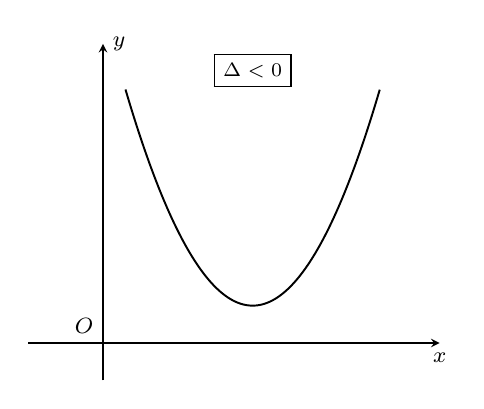
\begin{tikzpicture}[smooth,samples=300,scale=0.95,>=stealth,font=\footnotesize]
				\draw[->] (-1,0)--(4.5,0) node[below]{$x$};
				\draw[->] (0,-0.5)--(0,4) node[right]{$y$};
				\draw (0,0) node[above left]{$O$};
				\draw[line width=0.7pt,domain=0.3:3.7] plot(\x,{(\x)^2-4*(\x)+4.5});
				\node[below] at (2,4) {\fbox{\scriptsize$\Delta <0$}};
			\end{tikzpicture}\\
			\indammm{Đồ thị luôn nằm trên $Ox$.}
		\end{minipage}\hspace{2cm}
		\begin{minipage}{4cm}
			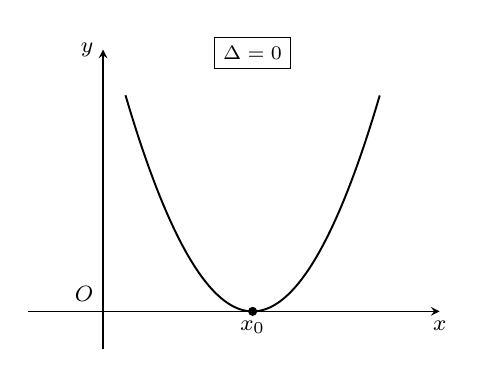
\begin{tikzpicture}[smooth,samples=300,scale=0.95,>=stealth,font=\footnotesize]
				\draw[->] (-1,0)--(4.5,0) node[below]{$x$};
				\draw[->] (0,-0.5)--(0,3.5) node[left]{$y$};
				\draw (0,0) node[above left]{$O$};
				\draw[line width=0.7pt,domain=0.3:3.7] plot(\x,{(\x)^2-4*(\x)+4});
				\draw[fill=black] (2,0) circle(1.5pt);
				\node[below] at (2,0) {$x_0$};
				\node[below] at (2,3.8) {\fbox{\scriptsize$\Delta =0$}};
			\end{tikzpicture}\\
			\indammm{Đồ thị nằm trên $Ox$ khi $x \ne x_0=-\frac{b}{2a}$.}
		\end{minipage}\hspace{2cm}
		\begin{minipage}{4cm}
			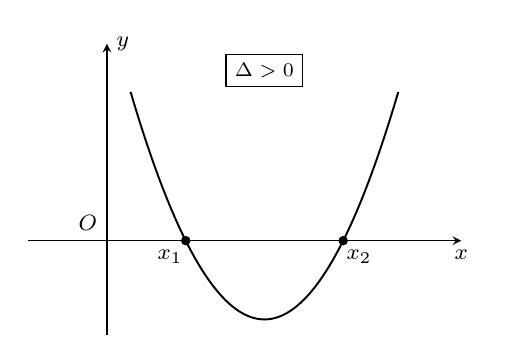
\begin{tikzpicture}[smooth,samples=300,scale=1,>=stealth,font=\footnotesize]
				\draw[->] (-1,0)--(4.5,0) node[below]{$x$};
				\draw[->] (0,-1.2)--(0,2.5) node[right]{$y$};
				\draw (0,0) node[above left]{$O$};
				\draw[line width=0.7pt,domain=0.3:3.7] plot(\x,{(\x)^2-4*(\x)+3});
				\draw[fill=black] (1,0) circle(1.5pt) (3,0) circle(1.5pt);
				\node[below] at (0.8,0) {$x_1$};
				\node[below] at (3.2,0) {$x_2$};
				\node[below] at (2,2.5) {\fbox{\scriptsize$\Delta >0$}};
			\end{tikzpicture}\\
			\indammm{Đồ thị nằm trên $Ox$ khi $x<x_1$ hoặc $x>x_2$; nằm dưới $Ox$ khi $x_1<x<x_2$.}
		\end{minipage}
	\end{center}
	
	\item [\iconCH] Nếu $a<0$:, ta có các trường hợp sau:
	\begin{center}
		\begin{minipage}{4cm}
			\begin{tikzpicture}[smooth,samples=300,scale=0.95,>=stealth,font=\footnotesize]
				\draw[->] (-1,0)--(4.5,0) node[below]{$x$};
				\draw[->] (0,-4)--(0,1) node[right]{$y$};
				\draw (0,0) node[below left]{$O$};
				\draw[line width=0.7pt,domain=0.3:3.7] plot(\x,{-(\x)^2+4*(\x)-4.5});
				\node[below] at (2,-2) {\fbox{\scriptsize$\Delta <0$}};
			\end{tikzpicture}\\
			\indammm{Đồ thị luôn nằm dưới $Ox$.}
		\end{minipage}\hspace{2cm}
		\begin{minipage}{4cm}
			\begin{tikzpicture}[smooth,samples=300,scale=0.95,>=stealth,font=\footnotesize]
				\draw[->] (-1,0)--(4.5,0) node[below]{$x$};
				\draw[->] (0,-3.5)--(0,1) node[left]{$y$};
				\draw (0,0) node[below left]{$O$};
				\draw[line width=0.7pt,domain=0.3:3.7] plot(\x,{-(\x)^2+4*(\x)-4});
				\draw[fill=black] (2,0) circle(1.5pt);
				\node[above] at (2,0) {$-\frac{b}{2a}$};
				\node[below] at (2,-2) {\fbox{\scriptsize$\Delta =0$}};
			\end{tikzpicture}\\
			\indammm{Đồ thị nằm dưới $Ox$ khi $x \ne x_0=-\frac{b}{2a}$.}
		\end{minipage}\hspace{2cm}
		\begin{minipage}{4cm}
			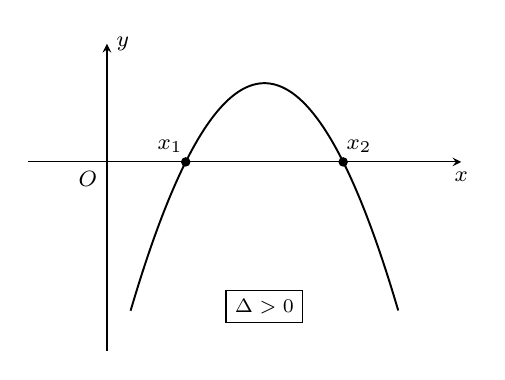
\begin{tikzpicture}[smooth,samples=300,scale=1,>=stealth,font=\footnotesize]
				\draw[->] (-1,0)--(4.5,0) node[below]{$x$};
				\draw[->] (0,-2.4)--(0,1.5) node[right]{$y$};
				\draw (0,0) node[below left]{$O$};
				\draw[line width=0.7pt,domain=0.3:3.7] plot(\x,{-(\x)^2+4*(\x)-3});
				\draw[fill=black] (1,0) circle(1.5pt) (3,0) circle(1.5pt);
				\node[above] at (0.8,0) {$x_1$};
				\node[above] at (3.2,0) {$x_2$};
				\node[below] at (2,-1.5) {\fbox{\scriptsize$\Delta >0$}};
			\end{tikzpicture}\\
			\indammm{Đồ thị nằm dưới $Ox$ khi $x<x_1$ hoặc $x>x_2$; nằm trên $Ox$ khi $x_1<x<x_2$.}
		\end{minipage}
	\end{center}
\end{itemize}

Tương ứng hình ảnh đồ thị ở trên, ta có bảng tổng kết dấu của tam thức bậc hai như sau:
\begin{itemize}
	\item [\iconCH] Nếu $a>0$:
	\begin{listEX}[3]
		\item [] \begin{tikzpicture}[scale=1,font=\footnotesize]
			\tkzTabInit[nocadre=false,lgt=1,espcl=2.5]
			{$x$ /0.6,$f(x)$ /0.6}
			{$-\infty$,$+\infty$}
			\tkzTabLine{,+,}
		\end{tikzpicture}
		\item [] \begin{tikzpicture}[scale=1,font=\footnotesize]
			\tkzTabInit[nocadre=false,lgt=1,espcl=1.4]
			{$x$ /0.6,$f(x)$ /0.6}
			{$-\infty$,$x_0$,$+\infty$}
			\tkzTabLine{,+,$0$,+,}
		\end{tikzpicture}
		\item [] \begin{tikzpicture}[scale=1,font=\footnotesize]
			\tkzTabInit[nocadre=false,lgt=1,espcl=1.2]
			{$x$ /0.6,$f(x)$ /0.6}
			{$-\infty$,$x_1$,$x_2$,$+\infty$}
			\tkzTabLine{,+,$0$,-,$0$,+,}
		\end{tikzpicture}
	\end{listEX}
	\item [\iconCH] Nếu $a<0$:
	\begin{listEX}[3]
		\item [] \begin{tikzpicture}[scale=1,font=\footnotesize]
			\tkzTabInit[nocadre=false,lgt=1,espcl=2.5]
			{$x$ /0.6,$f(x)$ /0.6}
			{$-\infty$,$+\infty$}
			\tkzTabLine{,-,}
		\end{tikzpicture}
		\item [] \begin{tikzpicture}[scale=1,font=\footnotesize]
			\tkzTabInit[nocadre=false,lgt=1,espcl=1.4]
			{$x$ /0.6,$f(x)$ /0.6}
			{$-\infty$,$x_0$,$+\infty$}
			\tkzTabLine{,-,$0$,-,}
		\end{tikzpicture}
		\item [] \begin{tikzpicture}[scale=1,font=\footnotesize]
			\tkzTabInit[nocadre=false,lgt=1,espcl=1.2]
			{$x$ /0.6,$f(x)$ /0.6}
			{$-\infty$,$x_1$,$x_2$,$+\infty$}
			\tkzTabLine{,-,$0$,+,$0$,-,}
		\end{tikzpicture}
	\end{listEX}
\end{itemize}

\begin{center}
	\begin{minipage}{8cm}
		\begin{tcolorbox}[colframe=cyan,colback=cyan!3,boxrule=0.2mm]
			\indamm{Định lý về dấu tam thức bậc hai:} Cho tam thức bậc hai $f(x)=ax^2+b x+c\,(a \neq 0)$.
			\begin{itemize}
				\item [\iconCH] Nếu $\Delta<0$ thì $f(x)$ cùng dấu với hệ số $a$ với mọi $x \in \mathbb{R}$.
				\item [\iconCH] Nếu $\Delta=0$ thì $f(x)$ cùng dấu với hệ số $a$ với mọi $x \neq-\frac{b}{2 a}$.
				\item [\iconCH] Nếu $\Delta>0$ thì tam thức $f(x)$ có hai nghiệm phân biệt $x_1$ và $x_2$ $\left(x_{1}<x_{2}\right)$. Khi đó, $f(x)$ cùng dấu với hệ số $a$ với mọi $x \in\left(-\infty ; x_{1}\right) \cup\left(x_{2} ;+\infty\right) ; f(x)$ trái dấu với hệ số $a$ với mọi $x \in\left(x_{1} ; x_{2}\right)$
			\end{itemize}
		\end{tcolorbox}
	\end{minipage}\hspace{0.5cm}
	\begin{minipage}{9cm}
		\begin{khung4}{Ghi nhớ dấu của $f(x)$ và $a$}
			\begin{itemize}
				\item[\iconCH] Nếu $\Delta < 0$ thì\\
				\begin{tikzpicture}
					\tkzTabInit[nocadre=false,lgt=1.2,espcl=4.2]
					{$x$ /0.7,$f(x)$ /0.8}
					{$-\infty$,$+\infty$}
					\tkzTabLine{,\text{cùng dấu },}
				\end{tikzpicture}
				\item[\iconCH] Nếu $\Delta = 0$ thì\\
				\begin{tikzpicture}
					\tkzTabInit[nocadre=false,lgt=1.2,espcl=2.5]
					{$x$ /0.7,$f(x)$ /0.8}
					{$-\infty$,$-\frac{b}{2a}$,$+\infty$}
					\tkzTabLine{,\text{cùng dấu },$0$,\text{ cùng dấu },}
				\end{tikzpicture}
				\item[\iconCH] Nếu $\Delta > 0$ thì\\
				\begin{tikzpicture}
					\tkzTabInit[nocadre=false,lgt=1.2,espcl=1.7]
					{$x$ /0.7,$f(x)$ /1}
					{$-\infty$,$x_1$,$x_2$,$+\infty$}
					\tkzTabLine{,\text{cùng dấu },$0$,\text{ trái dấu },$0$,\text{ cùng dấu },}
				\end{tikzpicture}
			\end{itemize}
		\end{khung4}
	\end{minipage}
\end{center}


\subsubsection{Bất phương trình bậc hai}
\begin{itemize}
	\item [\iconMT] \indam{Định nghĩa:} Bất phương trình bậc hai ẩn $x$ là bất phương trình có dạng $a x^{2}+b x+c>0$ (hoặc $\left.a x^{2}+b x+c \geq 0, a x^{2}+b x+c<0, a x^{2}+b x+c \leq 0\right)$, trong đó $a, b, c$ là những số thực đã cho và $a \neq 0$.
	\begin{boxkn}
		\begin{itemize}
			\item Số thực $x_{0}$ gọi là một nghiệm của bất phương trình bậc hai $a x^{2}+b x+c>0$, nếu $a x_{0}^{2}+b x_{0}+c>0$. Tập hợp gồm tất cả các nghiệm của bất phương trình bậc hai $a x^{2}+b x+c>0$ gọi là tập nghiệm của bất phương trình này.
			\item Giải một bất phương trình bậc hai là tìm tập nghiệm của nó.
		\end{itemize}
	\end{boxkn}
	\item [\iconMT] \indam{Một số kết quả cần nhớ:} Cho tam thức bậc hai $ax^2+bx+c$, với $a \ne 0$.
	\begin{listEX}[2]
		\item [\ding{172}]$ax^2+bx+c>0, \forall x\in \mathbb{R} \Leftrightarrow \left\{\begin{aligned}
			&a>0\\
			& \Delta <0.
		\end{aligned}\right.$
		\item [\ding{173}] $ax^2+bx+c<0, \forall x\in \mathbb{R} \Leftrightarrow \left\{\begin{aligned}
			&a<0\\
			& \Delta <0.
		\end{aligned}\right. $
		\item [\ding{174}] $ax^2+bx+c\geqslant 0, \forall x\in \mathbb{R} \Leftrightarrow \left\{\begin{aligned}
			&a>0\\
			& \Delta \leqslant 0.
		\end{aligned}\right. $
		\item [\ding{175}] $ax^2+bx+c\leqslant 0, \forall x\in \mathbb{R} \Leftrightarrow \left\{\begin{aligned}
			&a<0\\
			& \Delta \leqslant 0.
		\end{aligned}\right. $
	\end{listEX}
\end{itemize}
